\begin{document}
\begin{comment}

\chapter{Nomenclature}
Terminology presented alphabetically.
\begin{itemize}
\item ECEF - Earth Centered Earth Fixed. A rotating Cartesian coordinate system with origin at the center of the earth.
\item DOP - Dilution Of Position. A measurement of the geometric spread for the satellites used for producing the solution of the GNSS-receiver.
\item GALILEO - European GNSS, active since 2011.
\item GPS - Global Positioning System, USA GNSS, active since 1978.
\item LLA - Longitude, Latitude, Altitude. The spherical coordinate system defined in degrees West and North, as well as an altitude above a theoretical Spheroid. The standard used will determine the position of the origin.
\item MSE - Mean square error. Defined as $\frac{1}{n}\sum (x-\hat{x})^2$.
\item NED - North, East Down. A Cartesian coordinate system defined locally. The axes of the system will, as indicated by the name, point in the direction of the determined North, East and Down directions. The Down direction is that perpendicular to the horizon and towards the center of the earth.
\item RMSE - Root Mean Square Error. Square root of MSE
\item UERE - User equivalent range error. A measurement of the noise magnitude from the satellite signals.
\end{itemize}
\end{comment}
\chapter{Background}
This section explains the theory behind:
\begin{itemize}
\item Important coordinate frames for representation and their relationship.
\item How observations are made, modelled and the observation error sources.
\item How satellite positions are calculated
\item How a global position estimate and differenced relative estimates are calculated.
\item How satellite geometry influences the estimate.
\end{itemize}
\begin{comment}
\section{An introduction to satellite navigation systems and its utility}
The human presence in space began with the launching of the Soviet Union's Sputnik, closely followed by the USA's Explorer satellites in 1957 and 1958 respectively. Since then, many more launches of human-made objects into space have been performed, by several different countries. For the purpose of positioning there exists several systems in parallel, among them the US "Global Positioning System" (GPS), the Russian "Globalnaja Navigatsionnaja Sputnikovaja Sistema"[Latin transliteration] (GLONASS) and the Chinese \begin{CJK}{UTF8}{gbsn}北斗
\end{CJK}(Eng: Beidou) are arguably the most well known. The general name for those satellites used for navigation purposes is the "Global Navigation Satellite System" (GNSS).
\par
The use of GNSS-positioning has spread from its original military purpose to being an integrated part of many applications, both business and consumer-oriented. The usage of positioning through satellite navigation is today widely spread and has numerous applications, such as being present in many modern cellphones, ships and cars.
The advantages include its global usability for outdoors conditions as well as providing accuracy mostly within 5 meters at any time of the day \cite{posAccuracy}.
This may also lead to revolutions in many industries such as farming when tractors may work the field unsupervised \cite{garcianoglobal} or the potential for autonomous delivery of medical or customer goods using drones \cite{Patrik2019}. 
\par
In some applications, only the relative position between two units is of importance, e.g. for a ship docking or when landing on a platform. For this situation, the necessary precision may be much higher, meaning that the position error must be very small. Through the use of more advanced techniques than standalone positioning, relative position accuracy on a cm level or below has been proven achievable \cite{gao2004performance}. 
\end{comment}
\section{Navigation frames and Earth representation}
In order to navigate in a 3D-world, a set of three vectors need to be defined. There exist global frames which may be used for positioning anywhere, as well as local frames which are defined with directions and origin at an arbitrary point. There are several representation frames for a point in a GNSS application, among those a few notable ones are the Longitude-Latitude-Altitude (LLA), Earth-Centered-Earth-Fixed (ECEF) and North-East-Down representations (NED). All systems presented follow the rotation of the earth. It is also implied that the standard is based on the WGS84 system as it is the basis for GPS.\\
\textbf{LLA:}
The LLA-system is a spherical system, using the angular arguments degrees West of the Greenwich meridian, denoted $\lambda$ and North of the equator, denoted $\phi$, as well as a straight coordinate height over the surface of the earth. The altitude argument relies on a reference to the model of the earth applied, where 0 altitude implies being on the surface. \\
\textbf{ECEF:} The ECEF system is a Cartesian system, where the x and y-axes go through the equator with the x-axis pointing through the 0-meridian and the z-axis straight north.\\
\textbf{NED:} A NED-coordinate system is defined locally at an arbitrary point such that the axes point respectively straight in the North, East and down direction, where down implies towards the center of the earth.\\
\textbf{Elevation Azimuth:}
The Elevation-Azimuth system is a spherical system defined locally. The radius can also be introduced to turn it into a 3D system. Elevation implies the degrees above the horizon and Azimuth the degrees clockwise from the north direction. This works well for an origin at a low altitude as the zero degrees defined by the horizon will be perpendicular to the radial direction of the earth, but for a higher altitude the angle to the horizon will become negative and this frame may lose its utility.

\subsection{Coordinate frame transformation}
The different coordinate systems representations are illustrated in figure \ref{fig:CF}. The transformation between a point $B$ in an ECEF frame to a local NED-frame around a point $A$ is given by the matrix 
\begin{equation*}
\begin{bmatrix} n\\ e\\ d \end{bmatrix}=
\begin{bmatrix}
-\sin \phi cos \lambda & -\sin \phi \sin \lambda & \cos \phi \\
-\sin \lambda &\cos \lambda &0 \\
\cos \phi \cos \lambda & \cos \phi \sin \lambda & \sin \phi
\end{bmatrix}
\begin{bmatrix}
\Delta x \\ \Delta y \\ \Delta z
\end{bmatrix}
\end{equation*}
where $n,e,d$ represents the position in the local frame, $\lambda$ and $\phi$ the longitude and latitude angles of the point of transformation and $\Delta x, \Delta y,\Delta z$ the difference between points $A$ and $B$ in ECEF-coordinates.
\begin{figure}[!h]
\centering
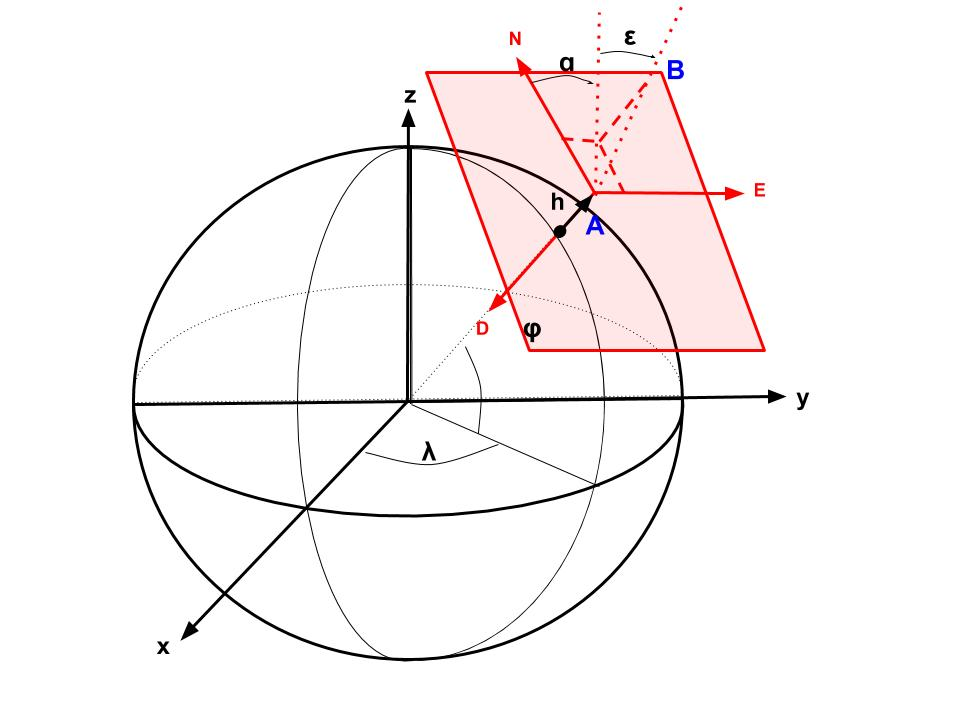
\includegraphics[width=0.8\textwidth]{Background/allCS}
\caption{\label{fig:CF} Commonly used coordinate frames for GNSS navigation and their correlation is shown. Global frames: ECEF, defined by directions x,y,z. LLA, defined by angles $\lambda, \phi$ and height $h$. Local frames around a point {\color{blue} \bf A} where the plane in red is tangential to the surface: NED, defined by the directions {\color{red} N,E,D}, and Elevation Azimuth for a point {\color{blue} \bf B} with regards to point {\color{blue} \bf A} given by $\alpha$ degrees clockwise from north and $\epsilon$ degrees above the horizon.}
\end{figure}

A special case of the rotation matrix which is that of the earth's rotation around its own axis should be mentioned. As this rotation coincides with the ECEF z-axis, it is a planar rotation which using basic algebra can be proven to be
\begin{equation}
\begin{bmatrix}\label{eq:rot_matrix}
\cos \lambda &\sin \lambda & 0 \\ 
-\sin \lambda & \cos \lambda & 0\\
0 & 0 & 1
\end{bmatrix}
\end{equation}
for a clockwise rotation $\lambda$. A property of the rotation matrix is that for any matrix $M(\lambda)$ defined by (\ref{eq:rot_matrix}), the inverse rotation is equivalent to its transpose $M(-\lambda)=[M(\lambda)]^T$.


\section{The pseudorange signal and error terms}\label{signalAndError}
The primary source of data for positioning is called the pseudorange and is based on calculating a time difference between transmission and reception which can be translated to a range through the speed of light. The specific method for measurement acquisition is based on sampling a sequence of the pseudorandom code sent out by a satellite, which is then compared for similarity to a longer sequence by the receiver. This gives the receiver information on when the signal was broadcast, while the time of reception is based on the receiver clock. Since in this project, the pseudorange will be sampled directly in the form of a distance from the receiver, the discussion on observation acquisition will not be explained further, more information on the specifics of how the signal is sampled can be found in \cite{Jeffrey}. 
\subsection{Components of the pseudorange} \label{pseudorangeComponents}
The pseudorange signal is measured as a time difference between time of transmission and reception. Both clocks times are assumed imperfect and containing an offset from the true time, which will impact the measurement. The measurement is considered a sum of three parts: the time difference between the true times of transmission and reception, the time difference between the respective clock offsets, and an error term \cite{6748618}. The model for these clock offsets are discussed further in section \ref{clockErrors}. The measured time of propagation, $T_{prop}$ is then expressed as
\begin{equation}\label{t_prop}
T_{prop}=(t_{rec}-t_{tr})+(\Delta t_{rec}-\Delta t_{sat})+\nu.
\end{equation}
where $t_{rec}$ and $t_{tr}$ are the true times of reception and transmission, $\Delta t_{sat}$ and $\Delta t_{rec}$ the transmitter and receivers respective offset from the true time in seconds and $\nu$ and error term, discussed further in section \ref{errorSources}. The propagation time for the signal is, with previously mentioned orbit, at around 6$\sim$7 ms and is the sought after component of the signal since it tells the distance to the sender. The measurement is transformed to a distance through multiplying with the speed of light $c$, and an observation can instead be expressed as a function of the actual distance and clock difference as
\begin{equation} \label{ObsRange}
y=||{\bf p}^{sat}-{\bf p}_{rec}||+c\Delta t+c\nu
\end{equation}
where ${\bf p}^{sat}$ and ${\bf p}_{rec}$ are the positions of the sender and receiver respectively. The use of bold font, e.g. $\bf p$ will be used forwards to indicate a vector. 
\par
The function $h$ defined as
\begin{align}\label{hModel}
h({\bf p}^{sat},{\bf p}_{rec},\Delta t_{rec}) &= ||{\bf p}^{sat}-{\bf p}_{rec}||+c\Delta t_{rec} \nonumber\\
				 &= \sqrt{\left((p^{sat}_x- p_x)^2+(p^{sat}_y-p_y)^2+(p^{sat}_z-p_z)^2\right)}+c\Delta t_{rec}.
\end{align}
is introduced, turning equation (\ref{ObsRange}) into
\begin{align} \label{singleObs}
y &=h({\bf p}^{sat}, {\bf p}_{rec},\Delta t_{rec})-c\Delta t_{sat} +c\nu\\
	&=h({\bf p}^{sat}, {\boldsymbol \theta })-c\Delta t_{sat} +c\nu.
\end{align}
The argument $\boldsymbol \theta=[{\bf p}_{rec},\Delta t_{rec}]$ has been introduced to represent the receiver state vector. The arguments of $h$ are the primary variables to estimate, but before the method to obtain an estimate can be explained, more underlying theory must be presented.

\subsection{Pseudorange error terms}
The different components of the error term $\nu$, mentioned in section \ref{pseudorangeComponents} are explained and given an expected range in this section. A summary of the noise sources can be found in table \ref{tableNoise}.
\subsubsection{Clock errors}\label{clockErrors}
The clocks in satellites are very precise, but as many of them have been active for a long time, the error can still amount to large values due to error build up over a long time. This error is called a bias and originates in the clock time advancing slightly different from an ideal clock, called a drift. This drift can be modeled as a random walk behavior and means that the error tends to build up slowly over time. The bias in receivers can often be much larger with a much higher drift. However between two consecutive samples, the difference is small, e.g.: an average drift of +1 second/day translates to $\sim10\mu s/s$. The clock biases give rise to a positioning error in two parts where the first part is the range error included in eq. (\ref{ObsRange}). These biases should be taken into account since a clock error of 1 ms can result in a positioning error of thousands of kilometers as 1 ms of clock bias equals to $c\cdot 0.001s\approx3\cdot 10^5$ m. 
\par
The second part of the clock bias positioning error stems from that the satellite position is determined with time as an argument, parametrized by a set of equations from the ephemeris data, explained more below. The receiver bias constitutes the largest part as an error in the receiver clock will lead to an error in the satellite position. The GNSS satellites travel at a speed of around 4000 m/s which means that a receiver clock error of $\Delta t_{rec}=0.01$ s can result in an error in the satellite position of around 40 m. Both the satellite and receiver clock errors will be compensated for, explained in section \ref{chap:ephPositioning} and \ref{stateEst}. The remaining error in the satellite clock after correction is in the range of 2.5 m \cite{Jeffrey}.

\subsubsection{Other error sources}\label{errorSources}
The third part of the signal, the noise terms $\nu$, is composed of several parts. This can be split up into a common noise and non common noise, where a common noise implies that it is equal for two simultaneous observations separate in space. If the common noise is expressed it will be denoted $\eta$. Otherwise, it will be included in the unmodelled noise sources, denoted $\epsilon$.
\par
The common noises include the Ionospheric and Tropospheric atmospheric noise, which can range up to 100 m \cite{IonoNoise} and 25 m \cite{williams2017tropospheric} respectively, but mostly are in the range of abut 5 m and 0.5 m respectively \cite{Jeffrey}. There are models for how to compensate for these effects, presented e.g. in \cite{Karaim2018Chapter4G} but they are not modeled in this project. Another common noise is the error in calculated position of the transmitting satellite, discussed further in section \ref{chap:ephPositioning}. The satellite position calculation is correct to in average 1 m in any direction \cite{satPos}. 
\par 
The unmodelled noise sources include multipath effects which is when signals are reflected of other objects, as well as receiver noise. These noise sources can be expected to be in the range of 1 and 0.3 m respectively \cite{Jeffrey}, but examples of multipath has been observed up to 100 m \cite{Karaim2018Chapter4G}.  

\begin{table}[h!]
  \begin{center}
    \begin{tabular}{|c|r|}\hline
		\textbf{Noise Source}& \textbf{Range} [m] \\      \hline
      	Satellite Clock & 	2.5 \\ \hline
		Satellite Orbit & 	1 \\ \hline
		Ionosphere & 		5 \\ \hline
		Troposphere&		0.5\\ \hline
		Multipath &			1 \\ \hline
		Receiver error & 	0.3 \\ \hline
    \end{tabular}
    \caption{\label{tableNoise} Noise sources in the range observations with a normal error range.}
  \end{center}
\end{table}

%\section{GNSS positioning} \label{ch:gnssPos}
%In this section, the method for determining the position of the satellites as well as some methods for obtaining a navigation solution through the information transmitted by the satellites are presented.
\section{Satellite positioning using ephemeris data}\label{chap:ephPositioning}
In order to determine a receiver's global position using satellites, the satellite's position should be known. The satellite positions at a given time are accessible online in real-time, e.g. from \url{gnssplanning.com} 
or can be calculated directly. The calculations are based on two parts: Almanac and ephemeris data. Almanac data is a predefined base orbit of lower accuracy which is updated on an approximately daily basis which is readily available online, e.g. on \url{https://www.navcen.uscg.gov/}
as well as satellites transmitting it directly. Precise positioning applications will rely on ephemeris data, which contains the parameters to calculate a more precise position of the satellite. This is transmitted by the individual satellite at a frequency of a few times per minute.
\par
The  data contained in the ephemeris message is based on the set of Keplerian equations which describes an orbit in space. 
%The information can vary between systems but is equal for GPS and Galileo which are the primary systems for observation here. In GPS and Galileo systems 
Each message will contain information of 20 parameters: two reference times, three clock correction factors, six Keplerian parameters and nine perturbation parameters. 
\par
The clock correction factors are specific to each satellite and are the primary form of clock correction, used to correct for the $\Delta t_{sv}$ term in (\ref{t_prop}). The equation to calculate the satellite clock bias, the precise algorithm for calculating the position and description of the Keplerian equations can be found in \cite{dunn2012global}. An example of the parameters in an ephemeris message used for this project is shown in figure \ref{fig:ephData}. The satellite position is then calculated using the corresponding ephemeris data with time as an argument and will be given in an ECEF frame.
\begin{figure}[!h]
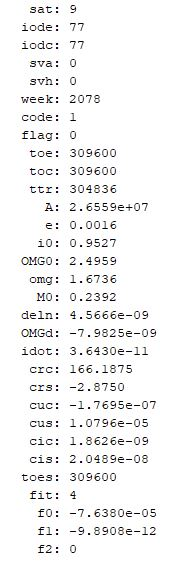
\includegraphics[scale=1]{Background/eph_values.jpg}
\caption{\label{fig:ephData} An example of a sample of the parameters contained in a single ephemeris message sampled on November 7, 2019.}
\end{figure}
\par 
It is relevant to note that the time applied in the GPS-system is zeroed at Midnight January 6, 1980, and expressed in the format number of weeks and time of the week in seconds, using midnight Sunday-Monday as reference.

\section{Global positioning model and estimates}
As each measurement is only given in one dimension, signals from several transmitters need to be taken into account in order to estimate the receiver's position. To estimate a position in 3D as well as the receiver clock bias a minimum of 4 transmitting satellites is needed. Utilizing the pseudorange measurements in combination with knowledge of the satellite's position at the time of transmission, a position estimate can be calculated. The receiver and satellite position are $3\times 1$-vectors $[x, y, z]$ conveniently expressed in an ECEF frame, as that is how satellite positions are given in calculations presented in section \ref{chap:ephPositioning}. To solve this with regards to the currently unknown $\boldsymbol \theta$, an iterative linearized solver can be implemented, presented below. For clarity, the values which are estimated and those calculated are as follows:

\paragraph{Estimates} The following are estimates in the model:
\begin{itemize}
\item ${\bf p}_{rec}$: Receiver position in [m] (ECEF), vector $1\times 3$.
\item $\Delta t_{rec}$: Receiver clock bias [s], scalar value.
\item ${\bf p}^{sat}$: Satellite position [m] at time of transmission (ECEF), vector $1\times 3$.
\item $\tau$: Time of flight [s] for GNSS-signal, scalar value.
\item $t$: Observation time, seconds of week in GPS-time [s] that signal was received by the receiver, scalar value.
\item $t_{tr}$: Time of transmission [s], scalar value.
\item $\gamma$: Earth's rotation [rad] during signal time of flight, scalar value.
\end{itemize}
\paragraph{Calculated or given values}
These values are either given or directly calculated given values.
\begin{itemize}
\item $y$: Pseudorange observation [m], scalar value.
\item $\Delta t_{sv}$: Satellite clock bias [s], scalar value.
\item $t_{rec}$: Nominal time of reception as registered by the receiver, not considering receiver clock bias, scalar value [s].
\item $\xi$: Ephemeris parameters, transmitted by each GNSS-satellite individually.
\item $\epsilon$: Unmodeled error source.
\end{itemize}
Any set of values or estimates will be ordered as a column vector, e.g. \textbf{y}=[y$^1$ ... y$^n$]$^T$ is a $n\times1$ vector of pseudorange observation, where a superscript is used as an index to indicate corresponding satellite and observation. 

\paragraph{Satellite position}
Satellite positions are calculated using the transmitted information in the ephemeris data as described in chapter \ref{chap:ephPositioning}. For a satellite, the position is calculated using only $t$ as an argument, and parametrized by the ephemeris values in $\xi$:
\begin{equation}\label{eq:p_sat}
{\bf p}^{sat}(t; \xi).
\end{equation}
\paragraph{Time of flight}
The time of flight is the propagation time of a signal between two arbitrary points $p_1$ and $p_2$. This is will be of relevance as the satellite position has changed between times t$_{tr}$ and $t$. It is calculated as
\begin{equation}\label{eq:tof}
\tau=\frac{1}{c}||{\bf p}_1-{\bf p}_2||
\end{equation}
\paragraph{Time of transmission}
Time of transmission for satellite signal is then calculated as 
\begin{equation}
t_{tr}=t-\tau.
\end{equation}
\paragraph{Earth's rotation}
The angle of rotation for a point on earth during $\tau$ seconds is given by 
\begin{equation}\label{eq:gamma}
\gamma=\tau\cdot\omega_e
\end{equation} 
\paragraph{Rotated satellite position}
Equations (\ref{eq:p_sat}-\ref{eq:gamma}) allow for calculating the position of a satellite at $t_{tr}$ as well as correcting for the rotation of the ECEF coordinate system during $\tau$ seconds. The satellite position is calculated at $t_{tr}$ and then rotated, resulting in the position ${\bf p}'(t_{tr};\gamma)$ in ECEF-coordinates is given by applying a rotation matrix to the position ${\bf p}^{sat}(t_{tr})$.
\begin{equation}\label{eq:coord_rotation}
{\bf p}'(t_{tr})=\begin{bmatrix} \cos(\gamma) &\sin(\gamma) &0\\  -\sin(\gamma) &\cos(\gamma)& 0\\ 0& 0 &1
\end{bmatrix}\left[{\bf p}^{sat}(t_{tr})\right]^T
\end{equation}
where the rotation applied is the counter clockwise rotation given by transposing (\ref{eq:rot_matrix}).
\paragraph{Satellite clock bias}
The satellite clock bias is calculated at nominal time $t_{rec}$ using the information in $\xi$ and considered a constant for a single observation.
\begin{equation} \label{estDtSV}
\Delta t_{sv}(t;\xi)
\end{equation}

\subsection{Global positioning observation model}
A single observation $y$ is modelled as 
\begin{align}
y&=h({\bf p}'(t_{tr}), {\boldsymbol \theta})-\Delta t_{sv}+\epsilon
\end{align}
which is the same as (\ref{singleObs}), with the exception that the satellite position is given by ${\bf p}'_{sat}$, given by equation (\ref{eq:coord_rotation}) and $\nu$ has been replaced by $\epsilon$ to indicate that it is not modelled. Thus the full model of an expected observation $\hat{y}$, given satellite position and receiver states is given by
\begin{align}\label{eq:obsModel}
\hat{y}=||{\bf p}'(t_{tr})-{\bf p}_{rec}(t)||+c\cdot(\Delta t_{rec}(t)-\Delta t_{sv})
\end{align}
where the unmodeled error $\epsilon$ is omitted.

\section{Global positioning estimator model}\label{stateEst}
The purpose of the equations presented above is to reach a solution for the receiver states ${\bf p}_{rec}$ and $\Delta t_{rec}$.
The actual implementation is an iterative process where estimates are updated until convergence. For the sake of presenting the governing model, any variable should be interpreted as the current estimate, which will then be updated at the next iteration until convergence is attained.
For a set of n observations ${\bf y}$ and the corresponding satellite positions $P^{sat}$ which is a $3\times n$ matrix, equation (\ref{singleObs}) can be expressed as:
\begin{align}
\textbf{y}&=h(P^{sat},{\boldsymbol \theta})+\Delta {\bf t}_{sv}+ {\boldsymbol \epsilon}\\
		  &=\begin{bmatrix} 
		  h^1({\bf p}^{(1)},{\boldsymbol \theta})\\ 
		  \vdots \\ 
		  h^n({\bf p}^{(n)},{\boldsymbol \theta}) \end{bmatrix} + \begin{bmatrix}
		  \Delta t_{sv}^1 \\ \vdots \\ \Delta t_{sv}^n
		  \end{bmatrix}+ \begin{bmatrix}
		  \epsilon_1 \\ \vdots \\ \epsilon_n
		  \end{bmatrix}
\end{align}
The satellite clock errors $\Delta {\bf t}_{sv}$ will be subtracted from the equations using the equation in \cite{dunn2012global} to get
\begin{align}
{\bf y}^*&=h({\bf p}^{sat},{\boldsymbol \theta})+ {\boldsymbol \epsilon}\\
		  &=\begin{bmatrix} 
		  h^1({\bf p}^{(1)},{\boldsymbol \theta})\\ 
		  \vdots \\ 
		  h^n({\bf p}^{(n)},{\boldsymbol \theta}) \end{bmatrix} +
		  \begin{bmatrix}
		  \epsilon_1 \\ \vdots \\ \epsilon_n
		  \end{bmatrix} \label{linearised}
\end{align}

The equations are solved for the estimate $\hat{\boldsymbol \theta}$ such that the error
\begin{equation}
||\textbf{y}^*-h(P^{sat},{\boldsymbol \theta})||^2
\end{equation} 
between observations and expected observations are minimized
\begin{align}\label{eq:thetaHat}
\hat{\bf \theta}=\operatorname*{argmin}_{\boldsymbol \theta}\left(||{\bf y}^*-h(P^{sat},{\boldsymbol \theta})||^2\right).
\end{align}
The system of equations is solved using the gradient of the equations. The gradient of the observation model equation (\ref{eq:obsModel}) is for a satellite $i$ 
\begin{align}
\frac{\partial}{\partial {\boldsymbol \theta}}h^{(i)}({\bf p}^{(i)},{\boldsymbol \theta})	&=
\frac{\partial h({\bf p}^{(i)},{\boldsymbol \theta})}{\partial x}+\frac{\partial h({\bf p}^{(i)},{\boldsymbol \theta})}{\partial y}+ \frac{\partial h({\bf p}^{(i)},{\boldsymbol \theta})}{\partial z}+\frac{\partial h({\bf p}^{(i)},{\boldsymbol \theta})}{\partial \Delta t} \nonumber \\
						&=-\frac{p^{(i)}_x-p_x}{||\bf p^{(i)}-p||}-\frac{p^{(i)}_y-p_y}{||\bf p^{(i)}-p||}-\frac{p^{(i)}_z-p_z}{||\bf p^{(i)}-p||}+c \nonumber \\
						:&=\nabla h^{(i)}({\bf p}^{(i)},{\boldsymbol \theta})\label{eq:nablaH}
\end{align}
All the gradients described by (\ref{eq:nablaH}) are collected in a $n\times 4$ matrix H:
\begin{align}\label{eq:H}
H(P^{sat},{\boldsymbol \theta})=\begin{bmatrix}
\nabla h^1({\bf p}^{1};{\boldsymbol \theta}) \\
\vdots \\
\nabla h^n({\bf p}^{n};{\boldsymbol \theta})
\end{bmatrix}.
\end{align}
The result of (\ref{eq:H}) leads to the least square solution of (\ref{eq:thetaHat}) being described by:
\begin{align}\label{eq:LS}
\hat{{\boldsymbol \theta}}=(H^T\cdot H)^{-1}H^T{\bf y}^*,
\end{align}
as described in \ref{ch:LS}. Equation \ref{eq:LS} is a step in a Gauss-Newton iterative process where a step is expressed as 
\begin{align*}
{\boldsymbol \theta}^{(j+1))}	& =
{\boldsymbol \theta}^{(j)}-\hat{{\boldsymbol \theta}}\\
				& =
{\boldsymbol \theta}^{(j)}-(H^T({\boldsymbol \theta}^{(j)})H({\boldsymbol \theta}^{(j)})^{-1}H^T({\boldsymbol \theta}^{(j)})({\bf y}- h\left[P^{sat, (j)},{\boldsymbol \theta}^{(j)}\right])
\end{align*}
where the superscript $(j)$ indicates an iteration number.\\
\subsection{Weighted estimator}\label{globalWEstimator}
If there is knowledge of the uncertainty in the observations, the minimizing function in \ref{eq:thetaHat} can be described by
\begin{align}\label{eq:theta_hatW}
\hat{{\boldsymbol \theta}}=\operatorname*{argmin}_{\bf \theta}\left(||{\bf y}-h(P^{sat},{\boldsymbol \theta})||^2_W\right).
\end{align}
where $||X||^2_W=X^TWX$ and $W$ is a matrix of weights, here it will always be assumed diagonal and non-negative. The so-called Best Linear Unbiased Estimator (BLUE) solution to equation (\ref{eq:LS}) will then be expressed as 
\begin{align}\label{eq:WLS}
\hat{{\boldsymbol \theta}}_{BLUE}=(H^T W H)^{-1}H^T W{\bf y}
\end{align}
As described in \ref{ch:WLS}.\\
In \cite{Brunner1999}, the signal-to-noise-ratio (SNR) value, which is closely related to the CNR and is recorded by the receivers is used as an estimate of the magnitude of the noise, such that the weight matrix will be described as a diagonal matrix $W=\text{diag}\left(w_1,\dots, w_n\right)$ 
for $n$ observations. A weight $w_i$, corresponding to observation $y^{(i)}$ and its corresponding registered SNR$^{(i)}$ value in dBHz are calculated as
\begin{equation}\label{SNRWeights}
w_i=10^{-0.1\cdot SNR^{(i)}}
\end{equation}
\subsection{Iterative steps of estimator}\label{iterativeModel}
The calculations to obtain (\ref{eq:thetaHat}) is in the order:
\begin{enumerate}
\item Calculate all $\Delta {\bf t}_{sv}$ for the satellites at time of reception $t$ and adjust the observations ${\bf y}^*= {\bf y} -\Delta {\bf t}_{sv}$. This step is not repeated.
\end{enumerate}
An epoch will be used to describe a set of observations made at the same instance and will be denoted by $[k]$.The final estimate, meaning the last iteration of the state estimates, will be denoted ${\boldsymbol \theta}[k]$. For the first epoch, $k=1$ The initial estimate of the receiver states ${\boldsymbol \theta}_0[1]$ is set to zero, i.e. ${\bf p}^{(0)}_{rec}[1]=[0, 0, 0]$ and $\Delta t^{(0)}_{rec}[1]=0$. For the subsequent epochs, $k>1$, the final estimate of the previous epoch is used as initial estimate, i.e. ${\boldsymbol \theta}_0[k+1]={\boldsymbol \theta}[k]$.
\begin{enumerate}
\setcounter{enumi}{1}
\item Adjust the observation for the receiver clock bias ${\bf y}^{**}={\bf y}*-c\Delta {\bf t}_{rec}$.\\
For each satellite individually:
\item Calculate signal time of flight $\tau^{(i)}=\frac{(\bf y^{(i)})**}{c}$ .
\item Calculate the satellite positions ${\bf p}^{(i)}(t_{rec}-\tau^{(i)};\xi)$.
\item Calculate the rotation angle $\gamma^{(i)}$.
\item Adjust the satellite position as in (\ref{eq:coord_rotation}) to obtain $({\bf p}^{(i)})'(t_{tr})$.
\item Calculate $\hat{{\boldsymbol \theta}}$ from ${\bf p}'(t_{tr})$, $\bf y^{**}$ and $\boldsymbol \theta$ as in equation (\ref{eq:LS}) or (\ref{eq:WLS}). 
\end{enumerate}
This is continued until convergence for steps 2-7, where the convergence threshold has been set to $10^{-3}$ m, indicating that
\begin{itemize}
\item The variables ${\bf y}^{**}$, $\boldsymbol \tau$, ${\bf p}_{rec}$ and $\Delta t_{rec}$ all are interdependent.
\item ${\bf p}^{sat}$, is dependant only on $\Delta t_{rec}$ and $\boldsymbol \tau$. 
\item $\boldsymbol \gamma$ is dependant only on $\boldsymbol \tau$.
\item $t$ is dependant only on $t_{rec}$ and $\Delta t_{rec}$.
\end{itemize}

\section{Estimator pseudo-code}
For the first epoch, the initial values of the receiver ${\boldsymbol \theta}_0[1]$ are set to 0. For any succeeding epoch $k>1$, the initial estimate of the states ${\boldsymbol \theta}_0[k]$ will use the final estimate of the previous epoch ${\boldsymbol \theta}[k-1]$. 
\par 
To calculate the receiver states during one epoch, all the estimated values are dependent on each other and any calculation will use the values calculated in the previous iteration of the others as input. In the code, the last iteration is denoted with a hat symbol, e.g. ${\bf \hat{p}}_{rec}$ and superscript is indexed by \texttt{(i)}. 
\par
The function "estimate\_satellite\_clock\_bias" is that from equation (\ref{estDtSV}). "get\_satellite\_position" comes from equation (\ref{eq:p_sat}). The rotation matrix in (\ref{eq:coord_rotation}) is represented by \texttt{R} and the "estimate\_position" function is the least squares solution to (\ref{eq:LS}). 
\par
In the following pseudo-code, the set of satellite positions $P_{sat}$ is a $n\times 3$ matrix, for a set of $n$ satellites where an index j relates to the corresponding satellite position ${\bf p}^{(j)}$. It is assumed that the set $\Xi=\{\xi^{(1)},\dots, \xi^{(n)}\}$ contains only the ephemeris data of the active satellites in each epoch.
\begin{algorithmic}
\STATE{1.Calculate satellite clock bias at observation time for each satellite}
\FOR{all j in $\Xi$}
\STATE{$\Delta {\bf t}_{sv}$(j)$\gets $estimate\_satellite\_clock\_bias(t, $\Xi$(j))}
\ENDFOR
\STATE{2. Adjust the observations for $\Delta {\bf t}_{sv}$}
\FOR{all j in $\Xi$}
\STATE{{\bf y}(j)$\gets$ {\bf y}(j)-$c\Delta {\bf t}_{sv}$(j)}
\ENDFOR
\STATE{$\Delta p \gets 100$ \\ $\Delta b \gets 100$}
\STATE{3.Iterate until convergence: calculate receiver states}
\WHILE{( $|\Delta p|\cup |\Delta b|$)>0.1}
\STATE{3.1 Calculate signal time of flight}
\FOR{all j in {\bf y}}
\STATE{{\bf y}(j) $\gets$ {\bf y}(j)-$c\Delta t_{rec}$}
\STATE{$\boldsymbol \tau$(j)$\gets$ {\bf y}(j)/$c$}
\ENDFOR
\STATE{3.2. Calculate the satellite position, rotation and rotated position}
\FOR{all j in $\Xi$}
\STATE{$P_{sat}$(j)$\gets$ get\_satellite\_position($\Xi$(j), t-$\boldsymbol \tau$(j))}
\STATE{$\boldsymbol \gamma$(j)$\gets \omega_e \cdot {\boldsymbol \tau}$(j)}
\STATE{$P_{sat}$(j)$\gets$ R($\boldsymbol \gamma$(j))$\cdot$ $P_{sat}$(j))}
\ENDFOR
\STATE{3.3 Estimate ${\bf p}_{rec}$ and $\Delta t_{rec}$}
\STATE{ $\hat{\bf p}$, $\Delta \hat{t}_{rec}\gets$ estimate\_position($P_{sat}$. {\bf y}, ${\bf p}_{rec}$, $\Delta t_{rec}$)}
\STATE{dp $\gets$ ${\bf p}_{rec}$- $\hat{\bf p}$}
\STATE{db $\gets$ $\Delta t_{rec}$-$\Delta \hat{t}_{rec}$}
\STATE{${\bf p}_{rec}\gets \hat{\bf p}$}
\STATE{$\Delta t_{rec} \gets \Delta \hat{t}_{rec}$}
\ENDWHILE
\end{algorithmic}
As it is a linearised system, the values of {\bf y},$\boldsymbol \tau$, ${\bf p}^{sat}$, $\boldsymbol \gamma$, ${\bf p}_{rec}$ and $\Delta t_{rec}$ will be updated per each iteration. This implies that for each iteration the position and receiver clock bias are estimated, and in turn the satellite position is adjusted for the updated clock bias value. This is repeated until convergence is reached.

\section{Relative positioning}\label{RelPos}
Relative positions can be calculated through the difference in positions calculated as in section \ref{iterativeModel} above. In this section a relative estimate using a DD-method is presented. The idea is to create an estimate of the relative distance between two positions by using the shared information between two receivers. It is based on that for two unit vectors ${\bf u}^{(i)}_a$ and ${\bf u}^{(i)}_b$ both pointing from receivers $a$ and $b$ respectively at position ${\bf p}_a$ and ${\bf p}_b$, to the same satellite at position ${\bf p}^{(i)}$ are considered to be parallel, as the angle $\alpha$ between ${\bf u}^{(i)}_a$ and ${\bf u}^{(i)}_b$ is very small. The idea is presented in figure \ref{fig:relPos}. This is motivated by that the satellite distance is generally much larger than the distance between any two points on earth, e.g. an isosceles triangle where the two receivers at a distance of 1 km and the satellite at a distance of $2\cdot 10^7$ m result in $\alpha$ being smaller than 0.05$^o$. The threshold for two observations considered close is set to 10 ms. If the observations are separated by more than that the entire epoch is discarded. 
\subsection{Differential technique observation model}
For the differential techniques presented below, the equation for a pseudorange measurement for the two receivers and a shared satellite $i$, at a given epoch will be:
\begin{align}
y^i_a&=\rho^{(i)}_a+c(\Delta t_a-\Delta t^{(i)})+\eta^i_a+\epsilon^i_a \label{Pa}\\
y^i_b&=\rho^{(i)}_b+c(\Delta t_b -\Delta t^{(i)})+\eta^i_b+\epsilon^i_b\label{Pb}
\end{align}
where $\rho^{(i)}_a$ indicates the distance between a satellite $i$ and receiver $a$.
\subsection{Single difference technique}\label{singleDifference}
In single difference technique, illustrated in figure \ref{fig:relPos}, the difference between two receivers is calculated, based on their relative distance to a satellite $i$, shown below when subtracting equation (\ref{Pb}) from (\ref{Pa}):
\begin{align*}
\Delta y^i_{ab}&=y^{(i)}_a-y^{(i)}_b\\
 		&=\rho^{(i)}_a+c(\Delta t_a-\Delta t^{(i)})+\eta^i_a+\epsilon^i_a\\
 		&-\rho^{(i)}_b+c(\Delta t_b -\Delta t^{(i)})+\eta^i_b+\epsilon^i_b\\
		&=(\rho^{(i)}_a-\rho^{(i)}_b)+c(\Delta t_a-\Delta t_b)-(\eta^i_a-\eta^i_b)+(\epsilon^i_a-\epsilon^i_b)\\
		&=\Delta \rho^{(i)}_{ab}+c\Delta t_{ab}+\Delta \eta^i_{ab}+\Delta \epsilon^i_{ab}
\end{align*}
As presented in \cite{blewitt1997basics}, with the same notation of $\Delta$ signifying a difference, this enables for the elimination of the satellite clock bias and orbit error, as well as atmospheric interference being effectively removed for receiver separations less than 30 km. Receiver clock bias should still be estimated.
\subsection{Double difference technique}
In order to remove the receiver clock bias, double difference can be implemented, illustrated in figure \ref{fig:relPosDD}. This relies on the difference between two satellites, $i$ and $j$, common between the two receivers. Introducing the symbol $\nabla$ to signify double difference, the equations is set up as
\begin{align}
\nabla \Delta y^{ij}_{ab}	&=\Delta y^{(i)} _{ab}-\Delta y^{(j)} _{ab} \nonumber \\
					&=\Delta \rho^{(i)}_{ab}+c\Delta t_{ab}+\Delta \epsilon^{(i)}_{ab}-\Delta \rho^{(j)}_{ab}-c\Delta t_{ab} -\Delta\epsilon^{(j)}_{ab} \nonumber\\
					&=\Delta \rho^{(ij)}_{ab}+\Delta\epsilon^{(ij)}_{ab}.\label{eq:DD}
\end{align}
In equation (\ref{eq:DD}) the receivers clock bias is eliminated. The atmospheric noise has been omitted as explained in section \ref{singleDifference}. Further, the relation between the relative position of two receivers is the dot product along a unit vector ${\bf e}^i=[e_x, e_y, e_z]$ pointing to a satellite $i$:
$$\Delta y^{(i)}_{ab}=\textbf{e}^i\cdot \textbf{r}_{ab}$$
and similarly, with a reference satellite $j$, the double difference distance is given by
$$\nabla \Delta y^{(ij)}_{ab}=(\textbf{e}^i-\textbf{e}^j)\cdot \textbf{r}_{ab}+\Delta\epsilon^{(ij)}_{ab}.$$
Thus, given a set of $n+1$ unit vectors pointing towards as many different satellites, and their corresponding pseudorange measurements, a solution can be found utilising equation (\ref{eq:LS}). Using satellite $j$ as reference, with its corresponding direction unit vector and observation as reference gives the following vectors
\begin{equation}\label{eq:DD-LS}
H=\begin{bmatrix} \textbf{e}^1-\textbf{e}^j\\ \vdots\\ \textbf{e}^{n}-\textbf{e}^j\end{bmatrix}, \hspace{0.5 cm}
\nabla \Delta \textbf{y}^{(j)}_{ab}=\begin{bmatrix}\Delta y^{1j}_{ab} \\ \vdots \\ \Delta y^{nj}_{ab} \end{bmatrix}.
\end{equation}
Equation \ref{eq:DD-LS} may be solved using the same least square method of \ref{eq:LS} as the global position, but with the updated direction matrix. 

\paragraph{Weighted least squares}
In \cite{BLUE} it is also suggested to use a BLUE estimator with the CNR in dBHz, denoted $\psi$, as an estimate of the noise level. The CNR value is registered by the receivers individually and is assumed inversely proportional to the variance of the noise of the observation $\sigma^2$. A higher variance shall result in a lower weight, formulated as that the variance of the noise for an observation between satellite $i$ and receivers $a$ and $b$ is given by
\begin{align*}
(\sigma^{(i)})^2&=(\sigma^{(i)}_a)^2+(\sigma^{(i)}_b)^2\\
		&\propto (\psi^{(i)}_a)^{-2}+(\psi^{(i)}_b)^{-2}.
\end{align*} 
The weight matrix $W$ is proposed as a diagonal weight matrix expressed as
\begin{equation}
W=\text{diag}\left(\frac{(\psi^1_a)^2\cdot(\psi^1_b)^2}{(\psi^1_a)^2+(\psi^1_b)^2},\dots,\frac{(\psi^n_b)^2\cdot \psi^n_b)^2}{(\psi^n_a)^2+(\psi^n_b)^2}\right)
\end{equation}
and the optimal solution is calculated as 
\begin{align*}
\hat{\boldsymbol \theta}_{BLUE}=\left((H^{(j)})^TWH^{(j)}\right)^{-1}(H^{(j)})^TW\nabla \Delta {\bf y}^{(j)}_{ab}
\end{align*} 
as proposed in equation (\ref{eq:WLS}), and $(H^{(j)})$ and $\nabla \Delta {\bf y}^{(j)}_{ab}$ are those presented in equation (\ref{eq:DD-LS}). Reference satellite $j$ is chosen to be the signal with the highest CNR value for each epoch. For these cases notable increase in accuracy is shown, compared to that of two global position estimates. 
\begin{figure}
\begin{minipage}[t]{0.48\textwidth}
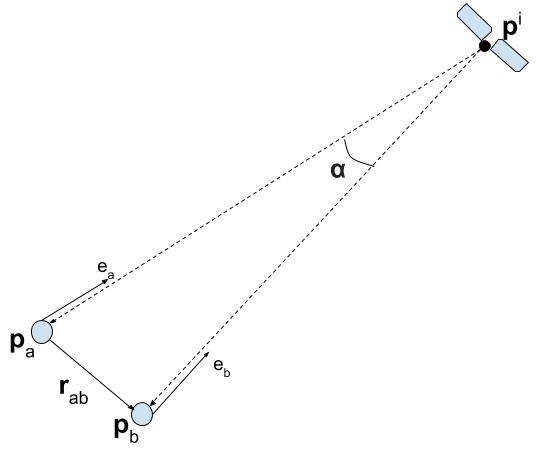
\includegraphics[width=\textwidth]{Background/relativePos}
\caption{\label{fig:relPos}Single difference technique is able to estimate a relative position as well as eliminating satellite clock bias.}
\end{minipage}
\hspace{1mm}
\begin{minipage}[t]{0.48\textwidth}
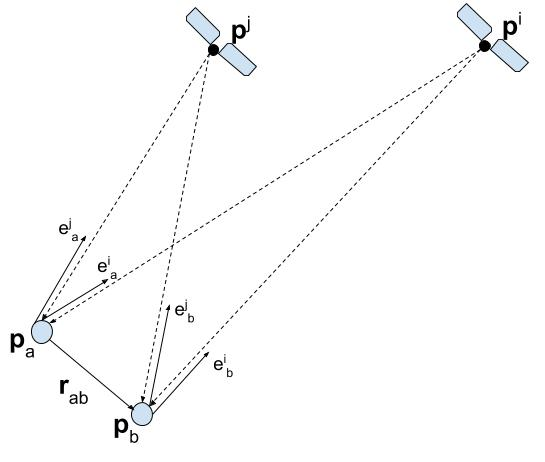
\includegraphics[width=\textwidth]{Background/relativePosDoubleDiff}
\caption{\label{fig:relPosDD}Satellite double difference can be calculated using two different satellites shared between the receivers}
\end{minipage}
\end{figure}

\section{Satellite Geometry}\label{satelliteGeometry}
One important aspect of the accuracy is in the spread of the satellites the receiver can obtain data from. If all observable transmitting satellites appear in a high angle over the horizon - as can be the case in an urban environment with many tall buildings - the accuracy can be expected to decrease compared to a case with more spread out satellite constellation. As all observations measure a distance in one direction, if all observable satellites are positioned close to being in the same direction, then distance estimates in other directions become poor. This is illustrated for an artificial 2D case in figure \ref{fig:DOPtheory}
\begin{figure}
\begin{minipage}[t]{0.5\textwidth}
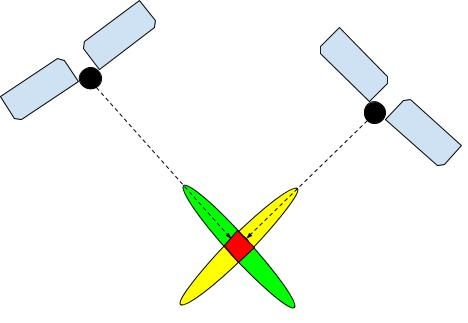
\includegraphics[width=\textwidth]{Background/LowDOP}
\end{minipage}
\begin{minipage}[t]{0.38\textwidth}
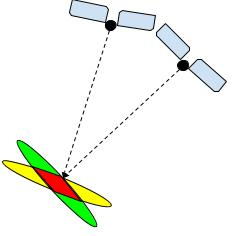
\includegraphics[width=\textwidth]{Background/HighDOP}
\end{minipage}
\caption{\label{fig:DOPtheory} Illustration of the accuracy based on satellite constellation. Areas of high probability perpendicular to each satellite intersect, with the high probability intersection area marked in red. In the left image the angles between the satellites is large creating a small region, while in the right image the small angle yields a larger area.}
\end{figure}
and is an effect of that close-lying points on a plane perpendicular to the radius all are approximately at the same distance from the center. 
\par 
In relation to this, the dilution of precision (DOP) can be defined. This is a matrix quantifying the geometric distribution of the satellites in use. Defining the matrix $Q=(H^TH)^{-1}$, where $H$ is the Jacobian of the geometric matrix in (\ref{linearised}) gives an estimate of the uncertainty of the solution per direction based on the geometry of the observed satellites. $q_{ij}$ is used to describe element row and column, the following definitions are commonly observed:
\begin{align}
HDOP=q_H&=\sqrt{q_{11}^2+q_{22}^2}\label{eq:HDOP}\\ 
VDOP=q_V&=q_{33}\label{eq:VDOP}\\ 
PDOP=q_P&=\sqrt{q_{11}^2+q_{22}^2+q_{33}^2}\label{eq:PDOP}\\ 
TDOP=q_T&=q_{44}\label{eq:TDOP}\\ 
GDOP=q_G&=\sqrt{q_{11}^2+q_{22}^2+q_{33}^2+q_{44}^2} \label{eq:GDOP}
\end{align}
Assuming that the geometric matrix is given in local NED coordinates, the HDOP, VDOP and PDOP respectively correspond to the horizontal, vertical and position uncertainty. TDOP is an estimate of the uncertainty in $\Delta t_{rec}$ and GDOP the geometric uncertainty. This gives an estimate of how noise in the observation maps to an error in the respective estimate. For this, the noise $\epsilon$ of each individual satellite should be assumed of equal magnitude \cite{tahsin2015analysis}. E.g. given a VDOP value of 3 and an error in the observations of 1 m, discussed in section \ref{signalAndError}, can be expected to result in a vertical error of 3m.
\par
The relation between satellite geometry and actual position uncertainty is expressed as a product of the noise level times the corresponding DOP value. 
\begin{equation}\label{UERE}
\sigma_X=\epsilon\cdot q_X
\end{equation}
The actual noise level in the observations, the sum of all error sources discussed in section \ref{signalAndError}, called the User Equivalent Range Error (UERE), is however usually not known to the receiver.
\par
The theoretically greatest achievable vertical spread is found with satellites under the receiver. This will not be achievable unless receiver is at a very high altitude since satellites below the horizon can't be observed. In practice an elevation threshold of at least 10$^o$ should be implemented since observations from low satellites have a higher noise level \cite{tatarnikov2014approaching}.
\par
This leads to that the horizontal spread is mostly much greater than the vertical and the HDOP-value can be expected to be smaller than the VDOP-value by a factor up to $\sim$2.5 \cite{langley1999dilution}. A GDOP value of 1 is considered ideal and should be considered good up to about 6 \cite{GDOPbelow6}.

\begin{comment}
\subsection{PDF, CDF and Conditional probability}
The probability density function (PDF) is the distribution over the state space, and is denoted $p(x=X)$ where $x$ is the variable and $X$ is the event, often the capital letter is omitted for brevity. A probability is always positive by definition. Since the probability of the all possible events equals 1, the cumulative distribution function CDF, denoted $P(x)$ is defined by the integral
\begin{align*}
P(x)&=\int_{-\infty}^{\infty}p(x)dx= 1.
\end{align*}
It is a non-decreasing function that must integrate to 1.

\subsection{Mean, variance and covariance}
With the previous definition of probability, three important concepts in statistical applications are introduced: the ideas of expectation, $E(\textbf{x})=\bar{x}$, variance: Var$(x)=\sigma^2_x$ and covariance Cov$(\textbf{x,y})=\Sigma_{xy}$ - easily confused with the symbol for sum, also often denoted $\Sigma$. Their discrete definitions are: 
\begin{align*}
\bar{x}&=\sum_x x\cdot p(x)= \frac{1}{N}\sum_{i=1}^N x_i\\
\sigma^2_x 		&=\sum_x (x-\bar{x})^2\cdot p(x) = E(x^2)-E(x)^2\\
\Sigma_{x,y} 	&=\sum_x \sum_y (x-\bar{x})(y-\bar{y})p(x,y) 
\end{align*}
and while the mean and variance are scalar values, describing the probability distribution of a single variable, the covariance will be a symmetric matrix where the diagonal elements are autocovariances. A property of importance of the covariance is that
\begin{align*}
\text{Var}(aX+bY)=a^2\text{Var}(X)+b^2\text{Var}(Y)+\text{Cov}(X,Y)
\end{align*} where $a$ and $b$ are scalars. This implies that if the variables $X$ and $Y$ are independent, meaning their covariance is 0, the variance always grows. The term bias is also important, where an unbiased estimate signifies a correct mean. E.g. for an actual value $\theta$ as introduced in \ref{stateEst} and its estimate $\hat{\theta}$, then $\hat{\theta}=\theta$, even if the variance may differ.
\end{comment}
\begin{comment}
\section{Filter models -ta bort helt?}
In order to manage the information coming from the different sensors, and creating a consistent solution, some sort of data fusing filter has to be implemented. This filter should make an estimate of the states based on some probabilistic assumptions and system dynamics as well as take the error into consideration. One assumption which will be made is the Markov assumption that a state $\bf x(t)$ is only dependant on the previous state $\textbf{x}(t-1)$. This means that the probability distribution is not dependent on previous measurements, or expressed mathematically: $$p(x(t)|x(t-1), x(t-2), \dots x(0))=p(x(t)|x(t-1))$$ where $p$ denotes a probability and $|$ a conditioning factor.
\subsection{Kalman filters}
The standard Kalman filter (KF) is the ideal filter given a linear state space as well as any unmodeled noise being Gaussian. The notion of a distribution being Gaussian is mathematically expressed as $$f(x|\mu,\sigma)= \frac{1}{\sqrt{2\pi\sigma^2}}e^{-\frac{1}{2\sigma^2}(x-\mu)^2}$$ for some mean value $\mu$ and a standard deviation $\sigma$. The property that the product of two Gaussians creates another Gaussian is very useful for this application and is used repeatedly. The Kalman filter consists of two steps:
\begin{enumerate}
\item Innovation - (also per Predict) the step where $\hat{\textbf{x}}(t|\textbf{x}(t-1), \textbf{u}(t))$ is calculated, and
\item Update - including sensor measurements $\textbf{x}(t|\textbf{z}(t),\bar{\textbf{x}}(t))$ 
\end{enumerate}
where the $\bar{x}$ notation indicates a state transition estimate and $\textbf{z}$ sensor measurements. The notation $x(t)$ is equivalent to $x_t$, as well as $x[k]$ is the same as $x_k$. These steps are performed at each time step according to the formula: \\
\textbf{Innovation:}
\begin{align*}
\bar{\textbf{x}}_t&=\text{A}_t \textbf{x}_{t-1}+\text{B}_t \textbf{u}_t\\
\bar{\Sigma}_t&=\text{A}\Sigma_{t-1}\text{A}^T+\text{R}_t\\
\end{align*}
followed by: \\
\textbf{Update:}
\begin{align*}
\text{K}_t&=\bar{\Sigma}_t \text{C}_t^T(\text{C}^T\bar{\Sigma}_t \text{C}_t^T+\text{Q}_t)^{-1}\\
\textbf{x}_t&=\bar{\textbf{x}}_{t}+\text{K}_t(\textbf{z}_t-\text{C}_t\bar{\textbf{x}}_t)\\
\Sigma_t&=(\text{I}-\text{K}_t\text{C}_t)\bar{\Sigma}_t
\end{align*}
The Q$_t$ and R$_t$ denotes the noise covariance matrices, which in the case of uncorrelated noise will be diagonal. Although nothing physical is never fully linear, for some applications they may be sufficiently small to be ignored. Since the vehicles in this project will be performing rotational movements the Kalman filter will be insufficient. A generalization of the (KF), the Extended Kalman Filter (EKF) implements a linearisation of the state space around the state estimate, mentioned in section \ref{linearisation}, which has been proven sufficient to deal with many more complex situations. SOURCE ON EKF. The iterative process will instead become:
\begin{align*}
\bar{\textbf{x}}_t&=g(\textbf{x}_{t-1},\textbf{u}_t)\\
\bar{\Sigma}_t&=\text{G}\Sigma_{t-1}\text{G}^T+\text{R}_t\\
\text{K}_t&=\bar{\Sigma}_t\text{H}_t^T(\text{H}_t\bar{\Sigma}_t\text{H}_t^T+\text{Q}_t)^{-1}\\
\textbf{x}_t&=\bar{\textbf{x}}+\text{K}_t(\textbf{z}_t-h(\bar{\textbf{x}_t}))\\
\Sigma_t&=(\text{I}-\text{K}_t\text{H}_t)\bar{\Sigma}_t
\end{align*}
Where the upper case matrices G$_t$ and H$_t$ represent the Jacobian of the functions $g$ and $h$ evaluated at $\bar{\textbf{x}}_t$.
\end{comment}

\end{document}
